% Using https://github.com/Kyslik/FEIstyle
\documentclass[dp]{FEIstyle}

%\usepackage{morewrites} % needed for minted
%\usepackage[newfloat]{minted}
%\usepackage{pdfpages}

\FEIauthor{Bc. Dávid Bednár}
\FEItitle{Tvorba užívateľského rozhrania k rozvrhovému systému pre FEI}
\FEItitleEn{GUI implementation for FEI schedule IS}
\FEIkeywords{rozvrhový systém, používateľské rozhranie, angular 5}
\FEIkeywordsEn{scheduling system, user interface, angular 5}
\FEIregNr{FEI-5384-46049}
\FEIsupervisor{Mgr. Ing. Matúš Jókay, PhD.}
%\FEIconsultant{Bc. Dávid Bednár}

\FEIglossaries{includes/glossary}
\bibliography{includes/bibliography.bib}

\iffalse \newacronym{acid}{ACID}{Atomicity, Consistency, Isolation, Durability}
\newacronym{ais}{AIS}{Akademický Informačný Systém}
\newacronym{ajax}{AJAX}{Asynchronous JavaScript And XML}
\newacronym{api}{API}{Application Programming Interface}
\newacronym{csrf}{CSRF}{Cross-site request forgery}
\newacronym{css}{CSS}{Cascading Style Sheets}
\newacronym{csv}{CSV}{Comma-separated values}
\newacronym{dom}{DOM}{Document Object Model}
\newacronym{dry}{DRY}{Don't Repeat Yourself}
\newacronym{fei}{FEI}{Fakulta Elektrotechniky a Informatiky}
\newacronym{gnu}{GNU}{GNU's not Unix}
\newacronym{hmac}{HMAC}{Hash-based Message Authentication Code}
\newacronym{html}{HTML}{HyperText Markup Language}
\newacronym{https}{HTTPS}{Hypertext Transfer Protocol Secure}
\newacronym{http}{HTTP}{Hypertext Transfer Protocol}
\newacronym{iana}{IANA}{Internet Assigned Numbers Authority}
\newacronym{id}{ID}{Identifikátor}
\newacronym{j2ee}{J2EE}{Java 2 Platform, Enterprise Edition}
\newacronym{json}{JSON}{JavaScript Object Notation}
\newacronym{js}{JS}{JavaScript}
\newacronym{jwt}{JWT}{JSON Web Token}
\newacronym{mptt}{MPTT}{Modified Pre-order Traversal Tree}
\newacronym{mvc}{MVC}{Model-View-Controller}
\newacronym{orm}{ORM}{Object-relational Mapping}
\newacronym{os}{OS}{Operačný Systém}
\newacronym{pdf}{PDF}{Portable Document Format}
\newacronym{rest}{REST}{Representational State Transfer}
\newacronym{rsa}{RSA}{RSA kryptosystém, iniciály jeho tvorcov}
\newacronym{spa}{SPA}{Single-page Application}
\newacronym{sql}{SQL}{Structured Query Language}
\newacronym{stu}{STU}{Slovenská Technická Univerzita v Bratislave}
\newacronym{tea}{TEA}{The Elm Architecture}
\newacronym{tls}{TLS}{Transport Layer Security}
\newacronym{ui}{UI}{User Interface}
\newacronym{uml}{UML}{Unified Modeling Language}
\newacronym{uri}{URI}{Uniform Resource Identifier}
\newacronym{url}{URL}{Uniform Resource Locator}
\newacronym{uim}{ÚIM}{Ústav informatiky a matematiky}
\newacronym{www}{WWW}{World Wide Web}
\newacronym{xml}{XML}{Extensible Markup Language}
\newacronym{xss}{XSS}{Cross-site scripting}
 \fi

\begin{document}
\frontmatter

\FEIpdfInfo
\FEIcover
\FEItitlePage

% \FEIassignment{includes/assignment_part2.jpeg}

% 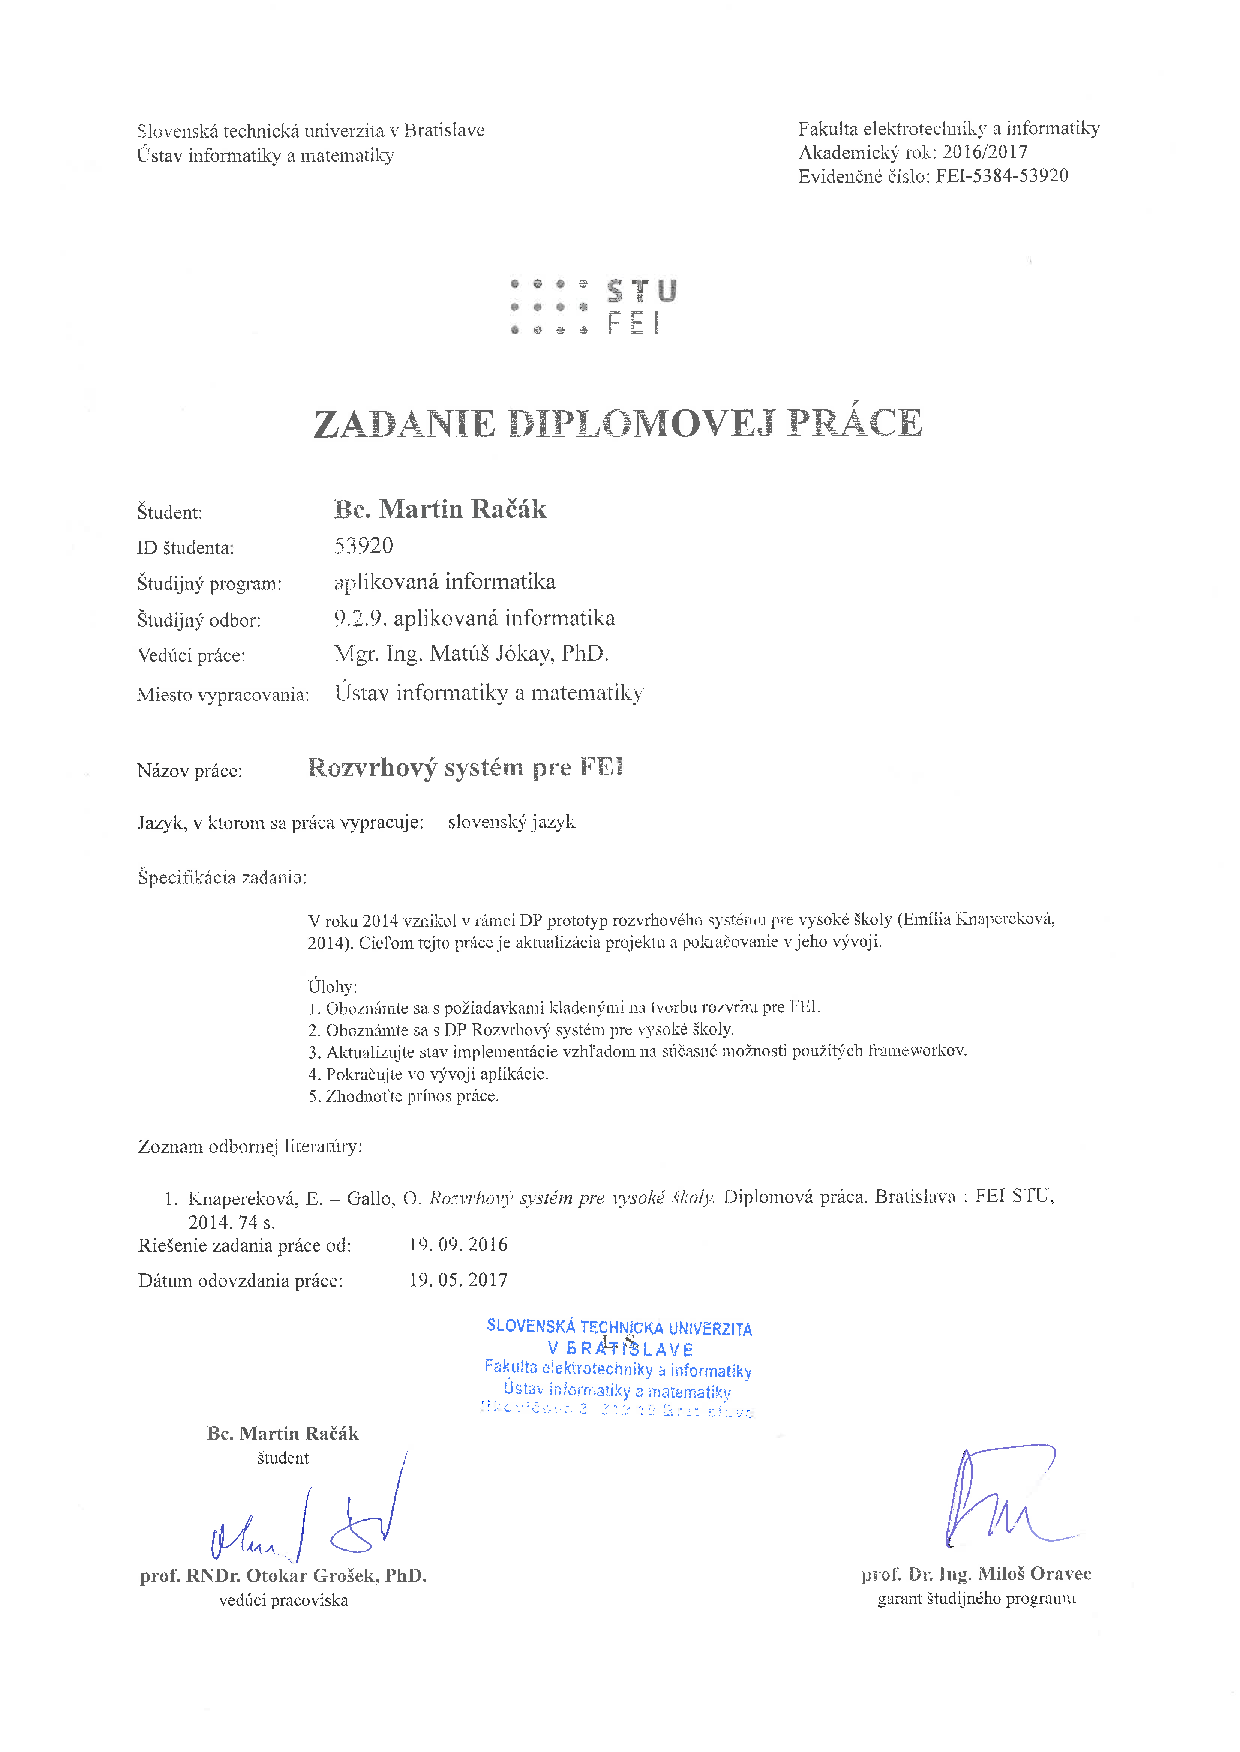
\includepdf{includes/assignment.pdf}
\FEIabstract{includes/abstract}
\FEIabstractEn{includes/abstractEN}
\FEIthanks{includes/thanks}
\FEIcontent
\FEIlistOfFiguresAndTables
% 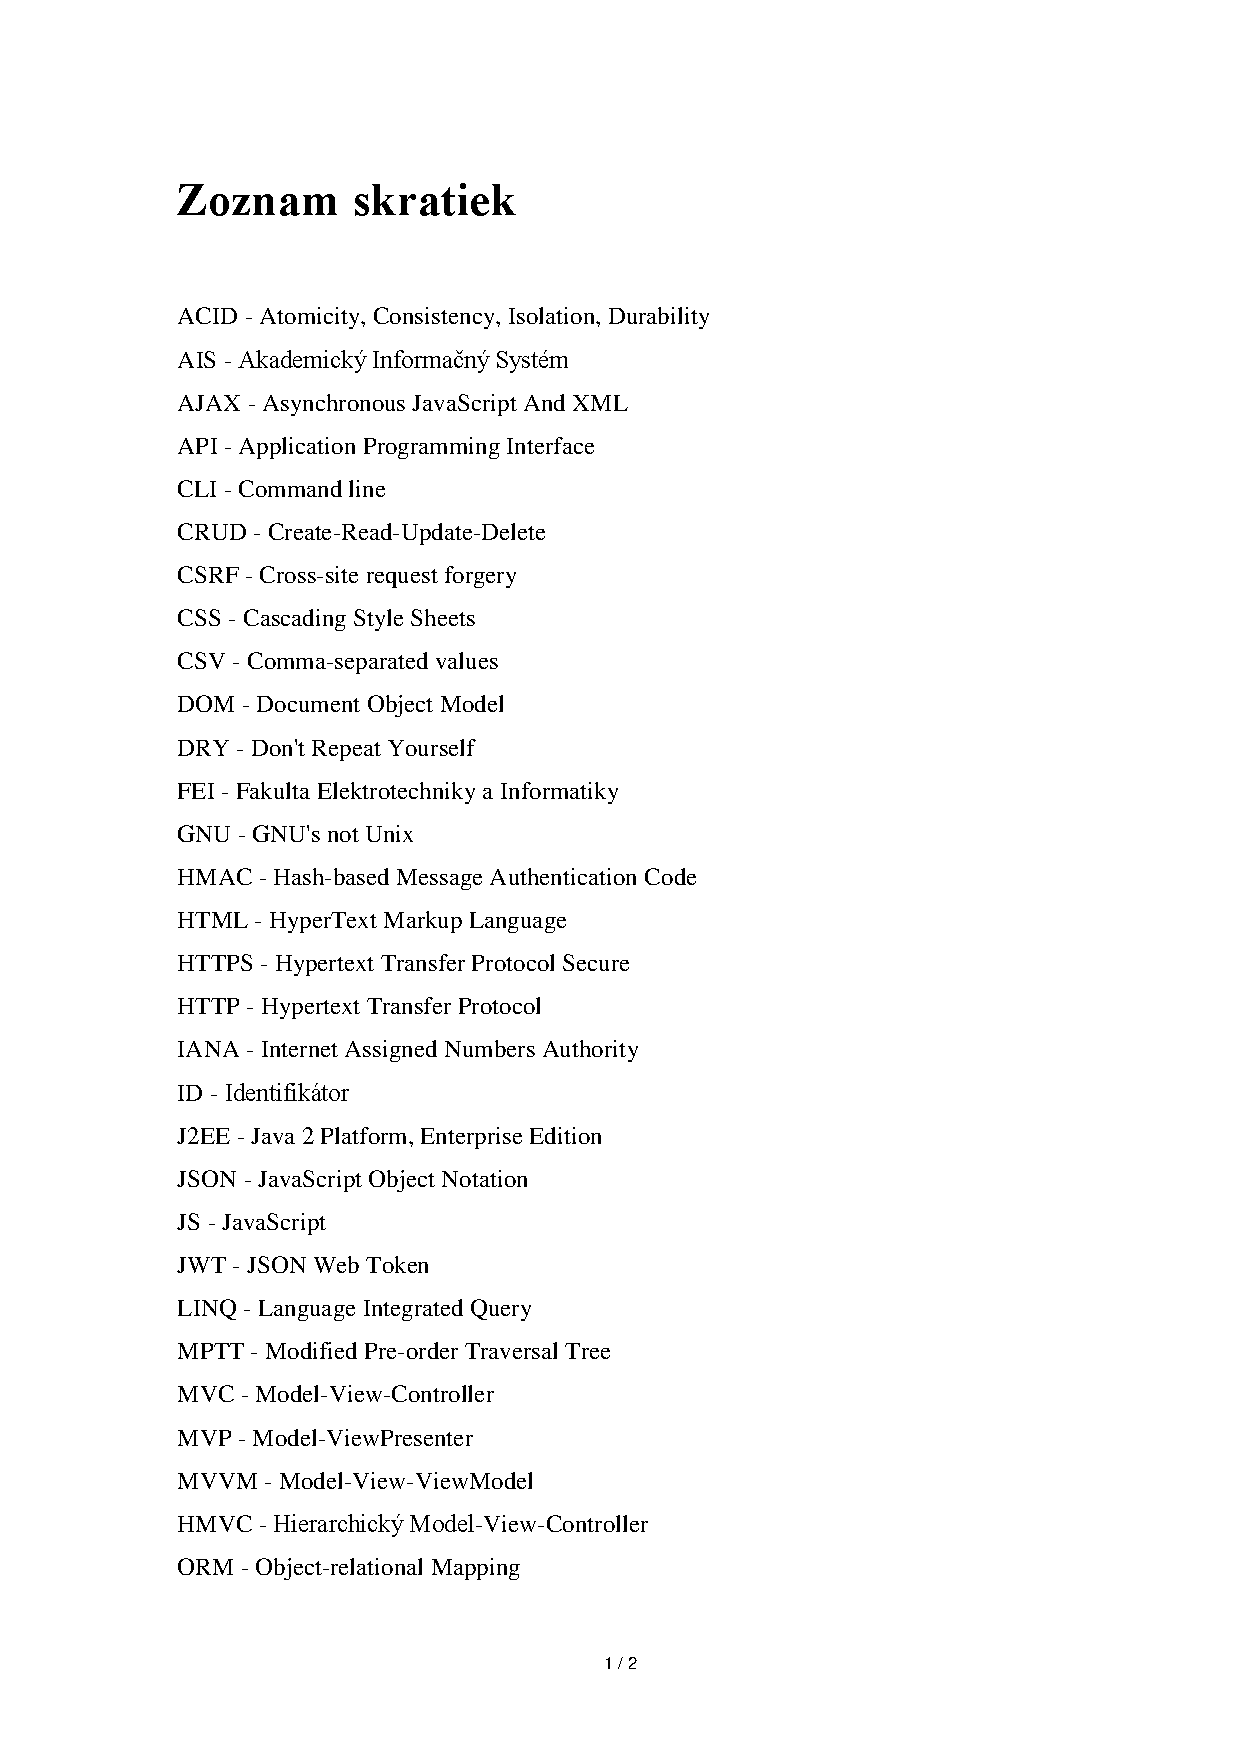
\includepdf{includes/glossary.pdf}
% \FEIlistOfGlossaries
% \FEIlistOfAlgorithms
% \FEIlistOfListings

\mainmatter

\FEIintroduction{includes/introduction}
\FEIcore{includes/core}
\FEIconclusion{includes/conclusion}
% \FEIresume{includes/resume} % Use only iff document is in english language

% bibliography should use UTF-8 accents (write as is ľščťžýáí...) NOT converted by BibDesk
% http://tex.stackexchange.com/questions/57743/how-to-write-%C3%A4-and-other-umlauts-and-accented-letters-in-bibliography
\FEIbibliography %includes/bibliography.bib

\backmatter

\FEIlistOfAppendix
\FEIappendix{Technická dokumentácia}{includes/technical-documentation}
\FEIappendix{Štruktúra elektronického nosiča}{includes/dir-structure}
%\FEIappendix{Štruktúra elektronického nosiča\label{att:A}}{includes/attachmentA}
%\FEIappendix{Algoritmus\label{att:B}}{includes/attachmentB}
%\FEIappendix{Výpis sublime\label{att:C}}{includes/attachmentC}
\end{document}